\documentclass[a4paper,12pt,leqno]{article} % добавить leqno в [] для нумерации слева

%%% Работа с русским языком
\usepackage{cmap}					% поиск в PDF
\usepackage{mathtext} 				% русские буквы в фомулах
\usepackage[T2A]{fontenc}			% кодировка
\usepackage[utf8]{inputenc}			% кодировка исходного текста
\usepackage[english,russian]{babel}	% локализация и переносы

%%% Дополнительная работа с математикой
\usepackage{amsmath,amsfonts,amssymb,amsthm,mathtools} % AMS
\usepackage{icomma} % "Умная" запятая: $0,2$ --- число, $0, 2$ --- перечисление

%% Номера формул
%%\mathtoolsset{showonlyrefs=false} % Показывать номера только у тех формул, на которые есть \eqref{} в тексте.

%% Шрифты
\usepackage{euscript}	 % Шрифт Евклид
\usepackage{mathrsfs} % Красивый матшрифт
\usepackage{graphicx}



\newtheorem{theorem}{Теорема}
\newtheorem{definition}{Определение}
\newtheorem{lemma}[theorem]{Лемма}

%% Перенос знаков в формулах (по Львовскому)
\newcommand*{\hm}[1]{#1\nobreak\discretionary{}
{\hbox{$\mathsurround=0pt #1$}}{}}




\begin{document} % конец преамбулы, начало документа

\begin{center}
    Федеральное государственное автономное образовательное учреждение
высшего образования

«Национальный исследовательский университет «Высшая школа экономики»
 Факультет компьютерных наук

Образовательная программа Прикладная математика и информатика
бакалавриат

\textbf{01.03.02 Прикладная математика и информатика} \linebreak[4]\vspace{5mm}

\textbf{ОТЧЕТ \\} 
 \textbf{по учебной практике}
\end{center}
\vspace{100mm}

\begin{flushright}
    Выполнил студент гр. БПМИ-185

    Агаев Фархат Чингизович
    

    \line(1,0){150}
\end{flushright}

\vspace{8mm}
\begin{flushleft}
    \textbf{Проверил:} \\
    Доцент Авдеев Роман Сергеевич
\end{flushleft}
\line(1,0){190} \; \; \; \line(1,0){115} \; \; \line(1,0){60} \\
\scriptsize{\textit{должность, ФИО руководителя от НИУ ВШЭ \; \; \; 
оценка по 10 бальной шкале \; \; \; \; \;подпись }
}

\newpage
\subsubsection*{Содержание}
\textbf{Введение...........................................................................................................................3}	

\noindent \quad Цели и задачи практики...................................................................................................................3 \\    

\noindent\textbf{Основная часть} 

\noindent\quad Календарный план-график...............................................................................................................4	\\

\noindent\quad Доказательство..................................................................................................................................5 \\

\noindent\quad Заключение.......................................................................................................................................11	\\

\noindent\quad Список использованных источников...............................................................................................11
\newpage
\subsubsection*{Введение}
\quad Для успешного прохождения практики "Дополнительные главы алгебры или линейной алгебры" 
\quad перед ее началом были обговорены цели, задачи, содержание и планируемые результаты, которые должны были быть достигнуты по завершении. 
\begin{itemize}
\item Главная цель:\\ 
\quad Доказать теорему Перрона-Фробениуса
\item Задачи практики: \\
1. Поиск необходимой информации в интернете и других источниках \\
2. Перевод доказательства с английского языка на русский \\ 
3. Написание подробного доказательства с использованием \LaTeX \\
\item Содержание практики (вопросы, подлежащие изучению): \\
1. Теорема Перрона \\
2. Теорема Перрона-Фробениуса\\
\item Планируемые результаты: \\
В результате практики должен быть подготовлен подробный качественнй pdf файл,
набранный в \LaTeX \\
\end{itemize}


\begin{figure}[p]
    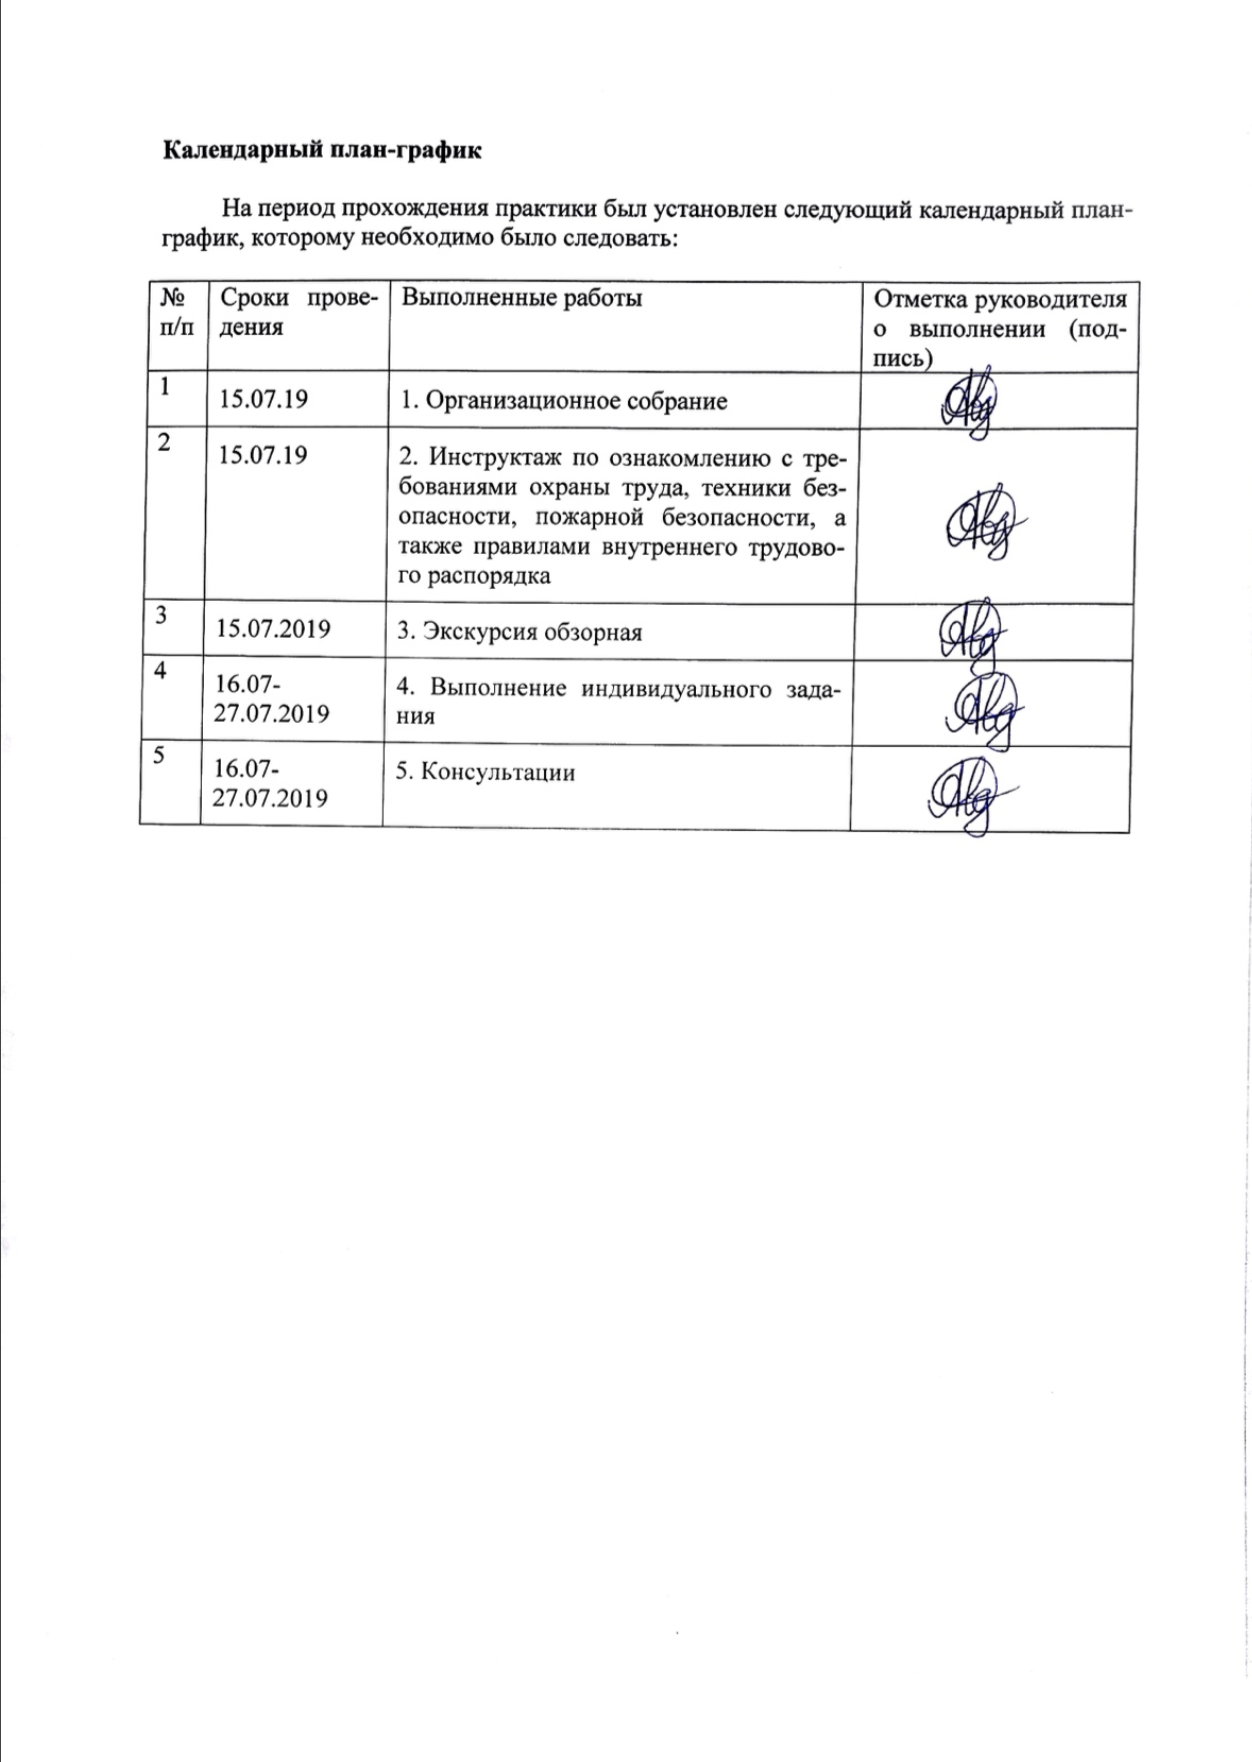
\includegraphics[scale=0.8]{1111.png}
\end{figure}

% \subsubsection*{Календарный план-график}
% \; \;На период прохождения практики был установлен следующий календарный план-график, 
% которому необходимо было следовать:

% \begin{tabular}{ | l | l | l | l | }
%     \hline
%     \begin{tabular}{cc} № \\
%     п/п  
%     \end{tabular}& Сроки прове-дения & Выполненные работы  &
%     \begin{tabular}{lll} Отметка руко - \\ водителя 
%         о выпол -  \\ нении 
%         (под-пись)  
%     \end{tabular}
%     \\ \hline
%     1 & 15.07.19 & \; 1. Организационное собрание  &  \\ \hline
%     2 & 15.07.19 &\begin{tabular}{l} 2. Инструктаж по ознакомлению с требованиями\\
%      охраны труда, техники безопасности, \\
%      пожарной безопасности,
%     а также \\ правилами внутреннего трудового распорядка \end{tabular}&  \\ \hline
%     3 & 15.07.2019 & \; 3. Экскурсия обзорная &  \\ \hline
%     4 & 16.07-27.07.2019 & \; 4. Выполнение индивидуального задания & \\ \hline
%     5 & 16.07-27.07.2019 & \; 5. Консультации & \\ \hline

%     \end{tabular}

\pagebreak    


\begin{definition}
    \textbf{Положительная матрица} - $A > 0$, когда каждый элемент $a_{ij} > 0$
\end{definition}

\begin{definition}
    \textbf{Неотрицательная матрица} - $A \geq 0$, когда каждый элемент $a_{ij} \geq 0$
\end{definition}


\begin{definition}
    \textbf{Спектральный радиус} 
    квадратной матрицы или линейного ограниченного оператора 
    является наибольшим абсолютным значениемего собственных значений 
    (т. e. Супремум среди абсолютных значений элементов в его спектре
    Иногда его обозначают как $\rho$ (·).
    Пусь $\lambda_1, \dotsc, \lambda_n $ (комплексные или действительные)
    \[\rho(A) = \max \left \{ |\lambda_1|, \dotsc, |\lambda_n| \right \}.\]
\end{definition}

\begin{definition}
    $\sigma(\textbf{A}) $ - множество различных собственных значений 
    матрицы А (спектр линейного оператора)
\end{definition}

\begin{definition}
    Матрица М абсолютных значений - \textnormal{\textbf{|M|}}, когда каждый элемент
    имеет значение $|m_{ij}|$, то есть при использовании операции \textnormal{|*|} 
    к матрице, мы применяем модуль к каждому её элементу
\end{definition}

\begin{definition}
    \textbf{Собственная пара} - пара $(\lambda, v)$, состоящая из собственного значения $\lambda$
     и соответствующему ему собственного вектора v.
\end{definition}

\begin{definition}
    \textbf{$alg \; mult_A(r)$} - Алгебраическая кратность корня $r$ для матрицы $А$.
\end{definition}

\begin{definition}
    \textbf{$geo \; mult_A(r)$} - Геометрическая кратность корня $r$ для матрицы $А$.
\end{definition}

\begin{definition}
    \textbf{Полупростое собственное значение} - собственное значение $\lambda$ с условием,
     что $geo \; mult_A(\lambda) = alg \; mult_A(\lambda)$
\end{definition}
\pagebreak

\section*{Положительные матрицы}
\subsection*{Простые утверждения}

Для начала приведем несколько очевидных фактов:
\begin{equation}
    A > 0 \Rightarrow \rho(A) > 0
\end{equation}
Предположим $\sigma(A) = \{0\}$, отсюда следует, что
жорданова форма для А и сама матрица А - нильпотент, но такое невозможно, так как $a_{ij} > 0$.
Также наше утверждение может быть ограничено до положительных матриц 
с спектральным радиусом 1, потому что A можно всегда нормализовать 
по спектральному радиусу, то есть $A > 0 \Leftrightarrow \frac{A}{\rho(A)} > 0 \text{ и } \rho(A) = 
r \Leftrightarrow \rho(\frac{A}{r}) = 1.$ 
\begin{align}
    P > 0 , x \geq 0, x \neq 0  &\Rightarrow Px > 0 \label{2} \\
    N \geq, u \geq v \geq 0  &\Rightarrow Nu \geq Nv \\
    N \geq 0, z > 0, Nz = 0  &\Rightarrow N =0, \\
    N \geq 0, n \neq 0, u > v > 0  &\Rightarrow Nu > Nv \label{5}
\end{align}
\begin{lemma}
    Если $A_{n \times n}$ > 0, то следующие утверждения верны:
    \begin{enumerate}
        \item $\rho(A) \in \sigma(A)$.
        \item Если $Ax=\rho(A)x$, тогда $A|x| = \rho(A)|x| $ и $|x| > 0$,
        другими словами для матрицы А существует собственная пара (опред №4)
        $(\rho(A), v)$, где v > 0
    \end{enumerate}
\end{lemma}
\noindent \textbf{Доказательство.} 
Как уже упоминалось ранее, мы можем предположить, 
что $\rho(A) = 1$ без ограничения общности.  Допустим, что у нас есть 
собственная пара $(\lambda, x)$ для матрицы А, где $|\lambda| = 1$, далее 
\begin{equation}
    |x| = |\lambda||x| = |\lambda x|= |Ax| \leq |A||x| = A|x| \Rightarrow |x| \leq A|x|.
\end{equation}
Цель состоит в том, чтобы показать, что равенство выполняется. Для удобства
пусть $z = A|x|$ и $y = z - |x|$ (по утверждению (6) мы знаем $y \geq 0$).
Предполагаем, что $y \neq 0, \; y_{i} > 0$. В этом случае из утверждения \eqref{2}
следует, что $Ay > 0$ и $z > 0$, поэтому должно существовать число $\varepsilon$
такое, что $Ay > \varepsilon z$ или эквивалентная запись, 
\begin{equation*}
    \frac{A}{1 + \varepsilon}z > z
\end{equation*}
Запишим данное неравеснство как $Bz > z$, где $B = \frac{A}{1 + \varepsilon}$
и последовательно умножаем с двух сторон на B используя утверждение \eqref{5}
мы получаем
\begin{equation*}
    B^2z > Bz > z, \quad B^3z > B^2z > z, \quad \dotsc \quad \Rightarrow B^kz > z
    \text{ для всех } k = 1, 2, \dotsc
\end{equation*} 
Но $\lim_{k \to \infty} B^k = 0$, потому что $\rho(B) = \sigma(\frac{A}{1 + \varepsilon}) =
\frac{1}{1 + \varepsilon} < 1$, поэтому в пределе мы получаем, 
что $0 > z$, который противоречит факту $z > 0$. Отсюда следует
ложное предположение $y \neq 0$, поэтому $y = 0 = A|x| - |x| \Rightarrow$
|x| - собсвтенный вектор для А с собсвтенным значеним $1 = \rho(A)$, 
заметим, что |x| = A|x| = z > 0 (ЧТД) \newline
Мы установили, что $\rho(A) > 0$  собственное значение для матрицы A > 0
\begin{lemma}
    Если $A_{n \times n} > 0$, то следующие утверждения верны:
    \begin{enumerate}
        \item $\rho(A)$ - единственное собственное значение на спектральном круге
        \item $\rho(A)$ - полупростое (опред №7) собственное значение.
    \end{enumerate}
\end{lemma}
\noindent\textbf{Доказательство.} 
Без ограничения общности $\rho(A) = 1$. Мы знаем из Леммы 1, что
если $(\lambda, x)$ - собственная пара для матрицы А $(|\lambda| = 1)$,
то $0 < |x| = A|x|$, так как 
$0 < |x_{k}| = (A|x|)_{k} = \sum^n_{j = 1}a_{kj}|x_{j}|$.
С другой стороны верно равенство 
$|x_{k}| = |\lambda||x_{k}| = |(\lambda x)_{k}|
 = |(Ax)_{k}| = |\sum^n_{j=1}a_{kj}x_{j}|$, 
\begin{equation}
    |\sum\limits_{j}a_{kj}x_{j}| = \sum\limits_{j}a_{kj}|x_{j}| = \sum\limits_{j}|a_{kj}x_{j}|
\end{equation}\label{7}
Для ненулевых векторов $\{z_{1}, \dotsc, z_{n}\} \in C^n,
 \| \sum_{j} z_{j} \|_{2} =  \sum_{j} \|z_{j} \|_{2}$
(факт) $\Leftrightarrow   z_{J} = \alpha_{j} z_{1} \text{ для некоторого } \alpha_{j} > 0$.
В частности это справедливо для скаляров, поэтому (7)
обеспечивает существование таких чисел $\alpha_{j} > 0$, 
\begin{equation*}
    a_{kj}x_j = \alpha(a_{k1}x_1) \text{ это эквивалентно } x_j = \pi_j x_1, \quad
    \pi_j = \frac{\alpha_ja_{k1}}{a_{kj}} > 0 
\end{equation*}
Другими словами, если $|\lambda| = 1, \;
  x = x_1p, \text{ где } p = (1, \pi_2, \dotsc, \pi_n)^T > 0$,
\begin{equation*}
    \lambda x = Ax \Rightarrow \lambda p = Ap = |Ap| = 
    |\lambda p| = |\lambda|p = p \Rightarrow \lambda = 1,
\end{equation*}
Таким образом 1 это единственное 
собственное значение на спектральном круге

\begin{lemma}
    \noindent Если матрицы $A_{n \times n} > 0$, 
    то следующие утверждения верны:
\end{lemma}
    \begin{enumerate}
        \item $alg \; mult_{A}(\rho(A)) = 1$ (Алгебраическая кратность равна 1)
        \item $dimN(A - \rho(A)I) = geo \; mult_{A}(\rho(A))$
        $ = alg \; mult_{A}(\rho(A)) = 1$ (опред №5 и №6)
    \end{enumerate}

\noindent\textbf{Доказательство.} 
    Без ограничения общности $\rho(A) = 1$ и 
    предположим, что $alg \; mult_{A} (\lambda = 1) = m > 1$.
    Мы уже знаем, что $\lambda = 1$ это \textbf{полупростое}
    собственное значение, которое означает, что $alg \; mult_{A}(1) = geo \; mult(1)$
    поэтому линейно независимые собственные вектора связаны с $\lambda = 1.$
    Если x и y - пара независимых собственных векторов соответствующих $\lambda = 1$,
    то $x \neq \alpha \text{ для всех } \alpha \in C$. Выберем ненулевой элемент из вектора y,
    пусть это будет $y_{i} \neq 0$ и установим что $z = x - \frac{x_i}{y_i}y.$ Поскольку $Az = z$  и мы знаем,
    из Леммы 1.2 $A|z| = |z| > 0.$ Но это противоречит условию
    $z_i = z_i - \frac{x_i}{y_i}y_i =0.$
    Следовательно предположение, что $m > 1$ неверно $\Rightarrow$ m = 1.

    Так как $N(A - \rho(A)I)$ - одномерное векторное пространство натянутый на некоторый
    $v > 0$, следовательно существует уникальный собственный вектор $p \in N(A - \rho(A)I)$
    такой, что $p > 0$ и $\sum_j p_j = 1 $(это получается с помощью нормализации $p = \frac{v}{\|v\|_1})$
    Данный вектор p называется \textbf{вектором Перрона} для матрицы $A > 0$ и ему соответствующее
    собственное значение $r = \rho(A)$ - \textbf{корень Перрона}.
    
    Поскольку $A > 0 \Leftrightarrow A^T > 0, \; \rho(A) = \rho(A^T)$ очевидно, что собственная пара (опред №4)
    $(r, p)$, которая существует для A, также существует пара (r, q) для $A^T$.
    Потому что $q^T A = r q^T$, вектор $q^T > 0$ называется \textbf{левым вектором Перрона}
    \begin{lemma}
     Вектор Перрона p - единственный для матрицы  $A_{n \times n} > 0$
    \end{lemma} 
    
    \noindent    \textbf{Доказательство.} 
    Если $(\lambda, y)$ это собственная пара для матрицы А, \newline
    $y \geq 0$ и если $ x > 0$ - вектор Перрона для $A_T$, тогда $x^Ty > 0$ (утвер.
    (2)), 
    \begin{equation*}
        \rho(A)x^T = x^TA \Rightarrow \rho(A)x^Ty = x^TAy = \lambda x^T y \Rightarrow \rho(A) = \lambda \quad \text{(ЧТД)}
    \end{equation*}
    
    \begin{lemma}
        Формула Коллатца – Виландта
    \end{lemma}
    Корень Перрона для матрицы $A_{n \times n} > 0, \; r = \max_{x \in N} f(x)$, где
    \begin{equation*}
        f(x) = \min_{1 \leq i \leq n}\frac{[Ax]_{i}}{x_i}, \; (x_i \neq 0), \quad N = \{x\; |\; x \geq 0,\; x \neq 0\}.
    \end{equation*}
    \noindent\textbf{Доказательство.} Если $\varepsilon = f(x)$ 
    для $x \in N$, тогда $0 \leq \varepsilon x \leq Ax$. 
    Пусть $p$ и $q^T$ будут соответственно правый и левый векторы Перрона для А с соответствующим
    корнем Перрона $r$ используем (3) (простые утверждения) вместе с утвер. (2) $(q^Tx > 0)$
    \begin{equation*}
        \varepsilon x \leq Ax \Rightarrow \varepsilon q^Tx \leq q^TAx = rq^Tx \Rightarrow
        \varepsilon \leq r \Rightarrow f(x) \leq r \quad \forall x \in N. 
    \end{equation*}
    Поскольку $f(p) = r$ и $ p \in N$, то $r = max_{x \in N}f(x).$ \newline
    Ниже приводится краткое изложение результатов, полученных выше
    \subsection*{Теорема Перрона}
    Соберем все леммы и утверждения, доказанные ранее, и получим теорему
     Перрона для положительных матрицы \newline
     \newline
     \textit{Если $A_{n \times n} > 0$, $ r = \rho(A)$, следующие утверждения верны.
    \begin{enumerate}
        \item $r > 0$
        \item $r \in \sigma(A)$ ($r$ называется корнем Перрона)
        \item $alg \; mult_{A}(r) = 1.$
        \item Существует собственный вектор $x > 0$ такой, что $Ax = rx$.
        \item Вектор $p$, который удовлетворяет условиям:
        \[ Ap = rp, \quad p > 0, \quad \|p\|_1 = 1\]
        называется вектором Перрона. Не существует других собственных векторов для матрицы А, кроме
        кратных $p$, не смотря на собственное значение.
        \item $r$ единсвтенное собственное значение на спектральном круге матрицы А
        \item Формула Коллатца-Виландта
        \begin{equation*}
            r = \max_{x \in N} f(x), \quad  f(x) = \min_{1 \leq i \leq n}\frac{[Ax]_{i}}{x_i}
        \end{equation*}
    \end{enumerate}
    }
    \section*{Неотрицательные матрицы}

    \begin{lemma}
        Пусть $A_{n \times n} \geq 0, \; r = \rho(A)$, то cледующие утверждения верны:
        \begin{enumerate}
            \item $r \in \sigma(A)$
            \item $Az = rz$ для $z \in N = \{x \, | \, x \geq 0, x \neq 0\}$
            \item Формула Коллатца-Виландта
            \begin{equation*}
                r = \max_{x \in N} f(x), \quad  f(x) = \min_{1 \leq i \leq n}\frac{[Ax]_{i}}{x_i}
            \end{equation*}
        \end{enumerate}
    \end{lemma}
    \textbf{Доказательство.} Рассмотрим последовательность положительных матриц 
    $A_k = A + \frac{1}{k}E > 0$, где  $E$ - единичная матрица, пусть $r_k > 0$ и $p_k > 0$
    отметим, что это корень Перрона и вектор Перрона соответственно для $A_k$.
    Заметим $\{p_k\}^{\infty}_{k = 1}$ - ограниченное множество, потому что 
    данное множество содержится в единичном шаре $\in \mathbb{R}^n$.
    Теорема Больцано — Вейерштрасса утверждает, что
    в ограниченной последовательности есть сходящаяся подпоследовательность, 
    поэтому в $\{p_k\}^{\infty}_{k = 1}$ мы 
    можем выделить сходящуюся подпоследовательность.
     
     $\{p_k\}^{\infty}_{k = 1} \rightarrow z$, где 
      $z \geq 0, \; z \neq 0 \text{ (потому что } p_{k_{i}} > 0, \; \|p_{k_{i}}\|_1 = 1)$
     Поскольку $A_1 > A_2 > \cdots > A,$ то $r_1 \geq r_2 \geq \cdots \geq r$,
     поэтому $\{r_k\}^\infty_{k=1}$ - монотонная последовательность с положительными 
     элементами, ограниченная $r$
     \begin{equation*}
        \lim_{k \to \infty} r_k = r^* \text{ существует, } r^* \geq r. \text{ В частности }
        \lim_{i \to \infty} r_{k_{i}} = r^* \geq r.
     \end{equation*}  
     Но $\lim_{k \to \infty} A_k = A \Rightarrow \lim_{i\to \infty} A_k = A$
     \begin{equation*}
        Az = \lim_{i \to \infty} A_{k_{i}}p_{k_{i}} = lim_{i \to \infty}r_{k_{i}}p_{k_{i}} =
        r*z \Rightarrow r* \in \sigma(A) \Rightarrow r* \leq r.
     \end{equation*}
     $\Rightarrow r* = r, Az = rz, z \geq 0, z \neq 0$ (доказали пункты 1 и 2 из Леммы 6).
     Докажем пункт 3. Пусть $q^T_k > 0$ будет левым вектором Перрона для матрицы $A_k$.
     Для каждого $x \in N$ и $k > 0$, мы знаем $q^T_kx > 0$ (прост утвержд 2), 
     \begin{align*}
        0 \leq f(x)x \leq Ax \leq Ax \leq A_kx \Rightarrow f(x)q^T_kx 
        \leq q^T_kA_kx=r_kq^T_kx \Rightarrow f(x) \leq r_k
        \\ \Rightarrow f(x) \leq r (r_k \rightarrow r^* = r).
     \end{align*} 
     $f(z) = r$ и $z \in N$, следовательно $max_{x \in N}f(x) = r$ \; (ЧТД)
     \begin{definition}
         $A_{n \times n}$ - \textbf{приводимая матрица}, когда существует перестановка
         матрицы P такая, что
         \begin{equation*}
            P^TAP = \begin{pmatrix}
                X & Y \\
                0 & Z
             \end{pmatrix},
             \; \text{где} \; X  \text{ и } Y \text{ - квадратные матрицы}
         \end{equation*}
         В противном случае матрица A - \textbf{неприводимая} 
     \end{definition}
    \subsection*{Теорема Перрона - Фробениуса (ч. 1)} 
    
    \textit{Если $A_{n \times n}$ - неприводимая матрица, то следующие утверждения верны: 
    \begin{enumerate}
            \item $r = \rho(A) \in \sigma(A) \; и \; r > 0$
            \item $alg mult_{A}(r) = 1$
            \item Cуществет собственный вектор x > 0, который удовлетворяет 
            условию Ax = rx.
            \item Вектор $p$, который удовлетворяет условиям:
            \[ Ap = rp, \quad p > 0, \quad \|p\|_1 = 1\]
            называется вектором Перрона. Не существует других собственных векторов для матрицы А, кроме
            кратных $p$, не смотря на собственное значение.
            \item Формула Коллатца-Виландта
            \begin{equation*}
                r = \max_{x \in N} f(x), \quad  f(x) = \min_{1 \leq i \leq n}\frac{[Ax]_{i}}{x_i}
            \end{equation*}
        \end{enumerate}    
    }
    \noindent\textbf{Доказательство.} Мы уже знаем из Леммы 6.2 
    $r = \rho(A) \in \sigma(A)$. Докажем, что $alg \; mult_A(r) = 1$,
    пусть $B = (I + A)^(n - 1) > 0$, будет матрица из Леммы 7. 
    Также мы знаем $\lambda \in \sigma(A) \Leftrightarrow (1 + \lambda)^{(n - 1)} \in \sigma(B),
    \quad alg \; mult_A(\lambda) = alg \; mult_B((1 + \lambda)^{n - 1})$.
    Вследствии этого если $\mu = \rho(B)$, то
    \begin{equation*}
        \mu = \max_{\lambda \in \sigma(A)}|(1 + \lambda)|^{n - 1} =
         \left\{\max_{\lambda \in \sigma(A)}|(1 + \lambda)|
         \right\}^{n - 1} = (1 + r)^{n - 1}
    \end{equation*}
    Потому что когда круглый диск $|z| \leq p$ переносится на одну единицу вправо,
    то точка максимума модулей в результирующем диске $|z + 1| \leq p$ это $z = 1 + p$
    (это очевидно, когда вы рисуете круг). $alg \; mult_A(r) = 1$. В противном случае 
    $alg \; mult_B(\mu) > 1$, но это невозможно так как $B > 0$. Чтобы 
    увидеть, что у А существует собственный вектор с собственным значением r, мы просто
    воспользуемся Леммой 7.2 и получим вектор $x \geq 0$ и $r$. Также довольно просто понять, что
    если $(\lambda, x)$ собственная пара для $А$, то $(f(\lambda), x)$ тоже собственная пара для А.
    Поэтому $(r, x)$  - собственная пара для А, предполагаем, что $(\mu, x)$ - собственная пара для $B$.
    С помощью Леммы 4 гарантируем, что $x$ должен быть положительным
     и кратным вектору Перрона для матрицы $B; \;$ $r > 0$; с другой стороны $Ax = 0$, 
     но это невозможно, так как $A \geq 0$ и $x > 0$, $Ax > 0$. 
     Довод также доказывает последние два пункта теоремы.

     
     \lemma{
         Если $A_{n \times n} \geq 0$ - неприводимая матрица 
         и имеет $h$ собственных значений 
         $\{\lambda_1, \lambda_2, \dotsc, \lambda_h$\} на спектральном круге
         то следующее условие верно:
         \begin{itemize}
            \item $alg \; mult_A(\lambda_k) = 1$ для $k = 1, 2, 3, \dotsc, h.$
         \end{itemize} 
     }

     \subsection*{Теорема Перрона - Фробениуса (ч. 2)}

     \textit{
        Если $A_{n \times n} \geq 0$ - неприводимая матрица 
        и имеет $h$ собственных значений 
        $\{\lambda_1, \lambda_2, \dotsc, \lambda_h$\} на спектральном круге,
         то
        \begin{itemize}
           \item $alg \; mult_A(\lambda_k) = 1$ для $k = 1, 2, 3, \dotsc, h.$
        \end{itemize}
        Если $A$ - примитивная матрица с $h$ собственными значениями на
        спектральном круге, то 
        \begin{itemize}
            \item $\sigma(A)$ - инвариантен при вращении 
            относительно начала координат на угол $2 \pi /h$.
        \end{itemize}  
     }
    
     \noindent\textbf{Доказательство.} Пусть $S = \{r, \; re^{i \theta_1, \dotsc, re^{i \theta_{h - 1}} }\}$
     - собственные значения на спектральном круге А. Мы знаем, что 
     \[A = e^{i \theta_k}D_kAD^{-1}_k \Rightarrow e^{i \theta_k}A \sim A
     \]
     Поэтому r - простое собственное значение для матрицы A (по теореме Перрона-Фробениуса),
     $re^{i \theta_k}$ также является простым собственным значением для матрицы 
     $e^{i \theta_k}A$. Но преобразование трансформации сохраняет собственные значения 
     и алгебраические кратности, поэтому $re^{i \theta_k}$ - собственное значение для матрицы A.
     Докажем пункт 2. 
     $\lambda \in \sigma(A) \Leftrightarrow \lambda e^{2 \pi i/h} \in \sigma(e^{2 \pi i/h}A)$ 
     , следовательно $\sigma(e^{2 \pi i/h}A) - \sigma(A)$, которая вращается на $2\pi/h$. Но из
     прошлого пунтка мы знаем, что матрицы  $A \sim e^{i \theta_k}A$, вследствии этого 
     $\sigma(A) = \sigma(e^{i \theta_k}A)$, следовательно возможен поворот на  $2\pi/h$. (ЧТД)


\newpage
\subsubsection*{Заключение}
Эта теорема имеет важные приложения к теории вероятностей (эргодичность цепей Маркова); 
теории динамических систем (подвиги конечного типа); 
в экономике (теорема Окисио, условие Хокинса - Саймона); 
к демографии (модель распределения населения по возрасту Лесли);
для социальных сетей (учебный процесс DeGroot), для поисковых систем в Интернете  
и даже для рейтинга футбольных команд.  Первым, кто обсудил порядок игроков в турнирах с использованием 
собственных векторов Перрона - Фробениуса, является Эдмунд Ландау.
\subsubsection*{Список использованных источников}
\begin{enumerate}
    \item Конспекты лекций
    \item https://www.emis.de/journals/MPRIA/2002/pa102i1/pdf/102a102.pdf
    \item https://epubs.siam.org/doi/pdf/10.1137/S0036144599359449 
\end{enumerate}
\end{document} % конец документа
